%By convention, white is front and blue is up
%Put white on right in diagrams, orange on left, blue up

\documentclass{article}
\usepackage{tikz}
\title{How to Solve a Rubik's Cube Like a Computer}
\date{}
\author{}
\newcommand{\drawtop}[9]{
	\coordinate (v0) at (0, 1);
	\coordinate (v1) at (-0.288675, 0.833333);
	\coordinate (v2) at (0, 0.666667);
	\coordinate (v3) at (0.288675, 0.833333);
	\coordinate (v4) at (-0.577350, 0.666667);
	\coordinate (v5) at (-0.288675, 0.5);
	\coordinate (v6) at (0, 0.333333);
	\coordinate (v7) at (0.288675, 0.5);
	\coordinate (v8) at (0.577350, 0.666667);
	\coordinate (v9) at (-0.866025, 0.5);
	\coordinate (v10) at (-0.577350, 0.333333);
	\coordinate (v11) at (-0.288675, 0.166667);
	\coordinate (v12) at (0.288675, 0.166667);
	\coordinate (v13) at (0.577350, 0.333333);
	\coordinate (v14) at (0.866025, 0.5);
	\coordinate (v15) at (0, 0);

	\fill[color = #1] (v0) -- (v1) -- (v2) -- (v3);
	\fill[color = #2] (v1) -- (v4) -- (v5) -- (v2);
	\fill[color = #3] (v4) -- (v9) -- (v10) -- (v5);
	\fill[color = #4] (v10) -- (v11) -- (v6) -- (v5);
	\fill[color = #5] (v5) -- (v6) -- (v7) -- (v2);
	\fill[color = #6] (v2) -- (v7) -- (v8) -- (v3);
	\fill[color = #7] (v7) -- (v13) -- (v14) -- (v8);
	\fill[color = #8] (v6) -- (v12) -- (v13) -- (v7);
	\fill[color = #9] (v11) -- (v15) -- (v12) -- (v6);

	%Left-Up diagonal lines
	\draw[color = black] (v9) -- (v0);
	\draw[color = black] (v10) -- (v3);
	\draw[color = black] (v11) -- (v8);
	\draw[color = black] (v15) -- (v14);

	%Down-Right diagonal lines
	\draw[color = black] (v0) -- (v14);
}

\newcommand{\drawleft}[9]{
	\coordinate (v0) at (-0.866025, 0.5);
	\coordinate (v1) at (-0.577350, 0.333333);
	\coordinate (v2) at (-0.288675, 0.166667);
	\coordinate (v3) at (0, 0);
	\coordinate (v4) at (-0.866025, 0.166667);
	\coordinate (v5) at (-0.577350, 0.0);
	\coordinate (v6) at (-0.288675, -0.166667);
	\coordinate (v7) at (0, -0.333333);
	\coordinate (v8) at (-0.866025, -0.166667);
	\coordinate (v9) at (-0.577350, -0.333333);
	\coordinate (v10) at (-0.288675, -0.5);
	\coordinate (v11) at (0, -0.666667);
	\coordinate (v12) at (-0.866025, -0.5);
	\coordinate (v13) at (-0.577350, -0.666667);
	\coordinate (v14) at (-0.288675, -0.833333);
	\coordinate (v15) at (0, -1);

	\fill[color = #1] (v0) -- (v1) -- (v5) -- (v4);
	\fill[color = #2] (v1) -- (v2) -- (v6) -- (v5);
	\fill[color = #3] (v2) -- (v3) -- (v7) -- (v6);
	\fill[color = #4] (v4) -- (v5) -- (v9) -- (v8);
	\fill[color = #5] (v5) -- (v6) -- (v10) -- (v9);
	\fill[color = #6] (v6) -- (v7) -- (v11) -- (v10);
	\fill[color = #7] (v8) -- (v9) -- (v13) -- (v12);
	\fill[color = #8] (v9) -- (v10) -- (v14) -- (v13);
	\fill[color = #9] (v10) -- (v11) -- (v15) -- (v14);
}

\newcommand{\drawright}[9]{
	\coordinate (v0) at (0, 0);
	\coordinate (v1) at (0.288675, 0.166667);
	\coordinate (v2) at (0.577350, 0.333333);
	\coordinate (v3) at (0.866025, 0.5);
	\coordinate (v4) at (0, -0.333333);
	\coordinate (v5) at (0.288675, -0.166667);
	\coordinate (v6) at (0.577359, 0.0);
	\coordinate (v7) at (0.866025, 0.166667);
	\coordinate (v8) at (0, -0.666667);
	\coordinate (v9) at (0.288675, -0.5);
	\coordinate (v10) at (0.577359, -0.333333);
	\coordinate (v11) at (0.866025, -0.166667);
	\coordinate (v12) at (0, -1);
	\coordinate (v13) at (0.288675, -0.833333);
	\coordinate (v14) at (0.577359, -0.666667);
	\coordinate (v15) at (0.866025, -0.5);

	\fill[color = #1] (v0) -- (v1) -- (v5) -- (v4);
	\fill[color = #2] (v1) -- (v2) -- (v6) -- (v5);
	\fill[color = #3] (v2) -- (v3) -- (v7) -- (v6);
	\fill[color = #4] (v4) -- (v5) -- (v9) -- (v8);
	\fill[color = #5] (v5) -- (v6) -- (v10) -- (v9);
	\fill[color = #6] (v6) -- (v7) -- (v11) -- (v10);
	\fill[color = #7] (v8) -- (v9) -- (v13) -- (v12);
	\fill[color = #8] (v9) -- (v10) -- (v14) -- (v13);
	\fill[color = #9] (v10) -- (v11) -- (v15) -- (v14);
}


\newcommand{\step}{\vspace{0.25cm}\hrule\vspace{0.25cm}}

\begin{document}

%%Template
\iffalse

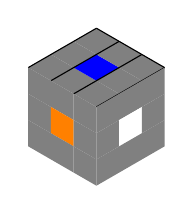
\begin{tikzpicture}[scale=1.0]
\drawtop{gray}{gray}{gray}{gray}{blue}{gray}{gray}{gray}{gray}
\drawleft{gray}{gray}{gray}{gray}{orange}{gray}{gray}{gray}{gray}
\drawright{gray}{gray}{gray}{gray}{white}{gray}{gray}{gray}{gray}
\end{tikzpicture}

\fi
%%

\maketitle
\newpage

%First step
Set \emph{solution number} to 0.

\step

%Orientation of 1st edge

\begin{center}
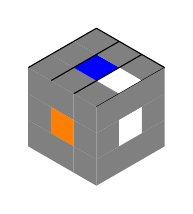
\begin{tikzpicture}[scale=1.0]
\drawtop{gray}{gray}{gray}{gray}{blue}{gray}{gray}{white}{gray}
\drawleft{gray}{gray}{gray}{gray}{orange}{gray}{gray}{gray}{gray}
\drawright{gray}{gray}{gray}{gray}{white}{gray}{gray}{gray}{gray}
\end{tikzpicture}
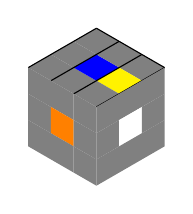
\begin{tikzpicture}[scale=1.0]
\drawtop{gray}{gray}{gray}{gray}{blue}{gray}{gray}{yellow}{gray}
\drawleft{gray}{gray}{gray}{gray}{orange}{gray}{gray}{gray}{gray}
\drawright{gray}{gray}{gray}{gray}{white}{gray}{gray}{gray}{gray}
\end{tikzpicture}
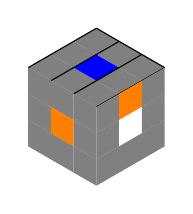
\begin{tikzpicture}[scale=1.0]
\drawtop{gray}{gray}{gray}{gray}{blue}{gray}{gray}{gray}{gray}
\drawleft{gray}{gray}{gray}{gray}{orange}{gray}{gray}{gray}{gray}
\drawright{gray}{orange}{gray}{gray}{white}{gray}{gray}{gray}{gray}
\end{tikzpicture}
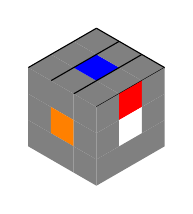
\begin{tikzpicture}[scale=1.0]
\drawtop{gray}{gray}{gray}{gray}{blue}{gray}{gray}{gray}{gray}
\drawleft{gray}{gray}{gray}{gray}{orange}{gray}{gray}{gray}{gray}
\drawright{gray}{red}{gray}{gray}{white}{gray}{gray}{gray}{gray}
\end{tikzpicture}
\end{center}

Add 1 to \emph{solution number}.

\step

%Orientation of 2nd edge

\begin{center}
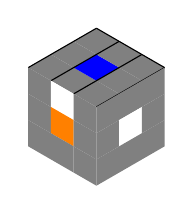
\begin{tikzpicture}[scale=1.0]
\drawtop{gray}{gray}{gray}{gray}{blue}{gray}{gray}{gray}{gray}
\drawleft{gray}{white}{gray}{gray}{orange}{gray}{gray}{gray}{gray}
\drawright{gray}{gray}{gray}{gray}{white}{gray}{gray}{gray}{gray}
\end{tikzpicture}
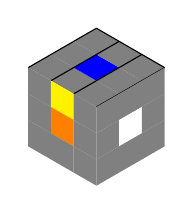
\begin{tikzpicture}[scale=1.0]
\drawtop{gray}{gray}{gray}{gray}{blue}{gray}{gray}{gray}{gray}
\drawleft{gray}{yellow}{gray}{gray}{orange}{gray}{gray}{gray}{gray}
\drawright{gray}{gray}{gray}{gray}{white}{gray}{gray}{gray}{gray}
\end{tikzpicture}
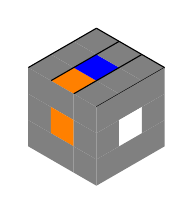
\begin{tikzpicture}[scale=1.0]
\drawtop{gray}{gray}{gray}{orange}{blue}{gray}{gray}{gray}{gray}
\drawleft{gray}{gray}{gray}{gray}{orange}{gray}{gray}{gray}{gray}
\drawright{gray}{gray}{gray}{gray}{white}{gray}{gray}{gray}{gray}
\end{tikzpicture}
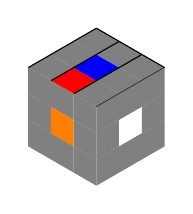
\begin{tikzpicture}[scale=1.0]
\drawtop{gray}{gray}{gray}{red}{blue}{gray}{gray}{gray}{gray}
\drawleft{gray}{gray}{gray}{gray}{orange}{gray}{gray}{gray}{gray}
\drawright{gray}{gray}{gray}{gray}{white}{gray}{gray}{gray}{gray}
\end{tikzpicture}
\end{center}

Add 2 to \emph{solution number}.

\step

%Orientation of 3rd edge

\begin{center}
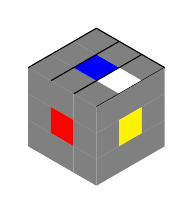
\begin{tikzpicture}[scale=1.0]
\drawtop{gray}{gray}{gray}{gray}{blue}{gray}{gray}{white}{gray}
\drawleft{gray}{gray}{gray}{gray}{red}{gray}{gray}{gray}{gray}
\drawright{gray}{gray}{gray}{gray}{yellow}{gray}{gray}{gray}{gray}
\end{tikzpicture}
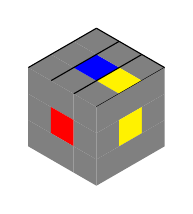
\begin{tikzpicture}[scale=1.0]
\drawtop{gray}{gray}{gray}{gray}{blue}{gray}{gray}{yellow}{gray}
\drawleft{gray}{gray}{gray}{gray}{red}{gray}{gray}{gray}{gray}
\drawright{gray}{gray}{gray}{gray}{yellow}{gray}{gray}{gray}{gray}
\end{tikzpicture}
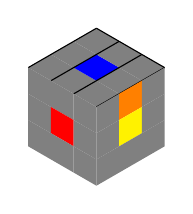
\begin{tikzpicture}[scale=1.0]
\drawtop{gray}{gray}{gray}{gray}{blue}{gray}{gray}{gray}{gray}
\drawleft{gray}{gray}{gray}{gray}{red}{gray}{gray}{gray}{gray}
\drawright{gray}{orange}{gray}{gray}{yellow}{gray}{gray}{gray}{gray}
\end{tikzpicture}
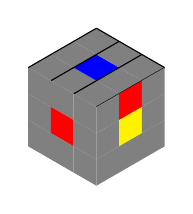
\begin{tikzpicture}[scale=1.0]
\drawtop{gray}{gray}{gray}{gray}{blue}{gray}{gray}{gray}{gray}
\drawleft{gray}{gray}{gray}{gray}{red}{gray}{gray}{gray}{gray}
\drawright{gray}{red}{gray}{gray}{yellow}{gray}{gray}{gray}{gray}
\end{tikzpicture}
\end{center}

Add 4 to \emph{solution number}.

\step

%Orientation of 4th edge

\begin{center}
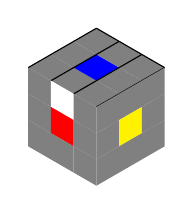
\begin{tikzpicture}[scale=1.0]
\drawtop{gray}{gray}{gray}{gray}{blue}{gray}{gray}{gray}{gray}
\drawleft{gray}{white}{gray}{gray}{red}{gray}{gray}{gray}{gray}
\drawright{gray}{gray}{gray}{gray}{yellow}{gray}{gray}{gray}{gray}
\end{tikzpicture}
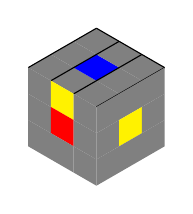
\begin{tikzpicture}[scale=1.0]
\drawtop{gray}{gray}{gray}{gray}{blue}{gray}{gray}{gray}{gray}
\drawleft{gray}{yellow}{gray}{gray}{red}{gray}{gray}{gray}{gray}
\drawright{gray}{gray}{gray}{gray}{yellow}{gray}{gray}{gray}{gray}
\end{tikzpicture}
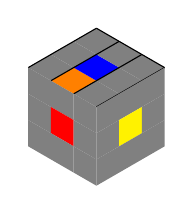
\begin{tikzpicture}[scale=1.0]
\drawtop{gray}{gray}{gray}{orange}{blue}{gray}{gray}{gray}{gray}
\drawleft{gray}{gray}{gray}{gray}{red}{gray}{gray}{gray}{gray}
\drawright{gray}{gray}{gray}{gray}{yellow}{gray}{gray}{gray}{gray}
\end{tikzpicture}
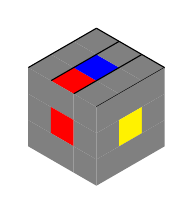
\begin{tikzpicture}[scale=1.0]
\drawtop{gray}{gray}{gray}{red}{blue}{gray}{gray}{gray}{gray}
\drawleft{gray}{gray}{gray}{gray}{red}{gray}{gray}{gray}{gray}
\drawright{gray}{gray}{gray}{gray}{yellow}{gray}{gray}{gray}{gray}
\end{tikzpicture}
\end{center}

Add 8 to \emph{solution number}.

\step

%Orientation of 5th edge

\begin{center}
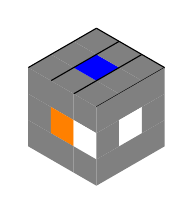
\begin{tikzpicture}[scale=1.0]
\drawtop{gray}{gray}{gray}{gray}{blue}{gray}{gray}{gray}{gray}
\drawleft{gray}{gray}{gray}{gray}{orange}{white}{gray}{gray}{gray}
\drawright{gray}{gray}{gray}{gray}{white}{gray}{gray}{gray}{gray}
\end{tikzpicture}
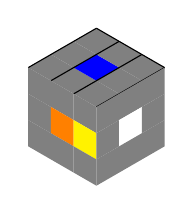
\begin{tikzpicture}[scale=1.0]
\drawtop{gray}{gray}{gray}{gray}{blue}{gray}{gray}{gray}{gray}
\drawleft{gray}{gray}{gray}{gray}{orange}{yellow}{gray}{gray}{gray}
\drawright{gray}{gray}{gray}{gray}{white}{gray}{gray}{gray}{gray}
\end{tikzpicture}
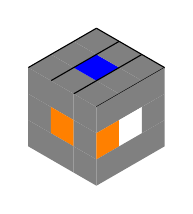
\begin{tikzpicture}[scale=1.0]
\drawtop{gray}{gray}{gray}{gray}{blue}{gray}{gray}{gray}{gray}
\drawleft{gray}{gray}{gray}{gray}{orange}{gray}{gray}{gray}{gray}
\drawright{gray}{gray}{gray}{orange}{white}{gray}{gray}{gray}{gray}
\end{tikzpicture}
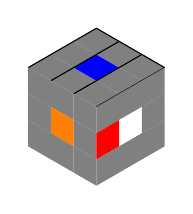
\begin{tikzpicture}[scale=1.0]
\drawtop{gray}{gray}{gray}{gray}{blue}{gray}{gray}{gray}{gray}
\drawleft{gray}{gray}{gray}{gray}{orange}{gray}{gray}{gray}{gray}
\drawright{gray}{gray}{gray}{red}{white}{gray}{gray}{gray}{gray}
\end{tikzpicture}
\end{center}

Add 16 to \emph{solution number}.

\step

%Orientation of 6th edge

\begin{center}
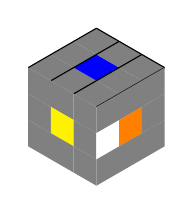
\begin{tikzpicture}[scale=1.0]
\drawtop{gray}{gray}{gray}{gray}{blue}{gray}{gray}{gray}{gray}
\drawleft{gray}{gray}{gray}{gray}{yellow}{gray}{gray}{gray}{gray}
\drawright{gray}{gray}{gray}{white}{orange}{gray}{gray}{gray}{gray}
\end{tikzpicture}
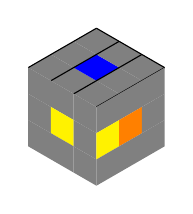
\begin{tikzpicture}[scale=1.0]
\drawtop{gray}{gray}{gray}{gray}{blue}{gray}{gray}{gray}{gray}
\drawleft{gray}{gray}{gray}{gray}{yellow}{gray}{gray}{gray}{gray}
\drawright{gray}{gray}{gray}{yellow}{orange}{gray}{gray}{gray}{gray}
\end{tikzpicture}
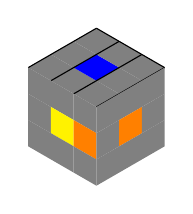
\begin{tikzpicture}[scale=1.0]
\drawtop{gray}{gray}{gray}{gray}{blue}{gray}{gray}{gray}{gray}
\drawleft{gray}{gray}{gray}{gray}{yellow}{orange}{gray}{gray}{gray}
\drawright{gray}{gray}{gray}{gray}{orange}{gray}{gray}{gray}{gray}
\end{tikzpicture}
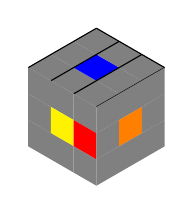
\begin{tikzpicture}[scale=1.0]
\drawtop{gray}{gray}{gray}{gray}{blue}{gray}{gray}{gray}{gray}
\drawleft{gray}{gray}{gray}{gray}{yellow}{red}{gray}{gray}{gray}
\drawright{gray}{gray}{gray}{gray}{orange}{gray}{gray}{gray}{gray}
\end{tikzpicture}
\end{center}

Add 32 to \emph{solution number}.

\step

%Orientation of the 7th edge

\begin{center}
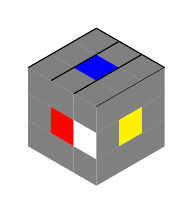
\begin{tikzpicture}[scale=1.0]
\drawtop{gray}{gray}{gray}{gray}{blue}{gray}{gray}{gray}{gray}
\drawleft{gray}{gray}{gray}{gray}{red}{white}{gray}{gray}{gray}
\drawright{gray}{gray}{gray}{gray}{yellow}{gray}{gray}{gray}{gray}
\end{tikzpicture}
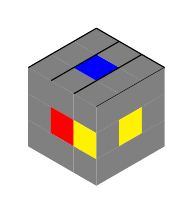
\begin{tikzpicture}[scale=1.0]
\drawtop{gray}{gray}{gray}{gray}{blue}{gray}{gray}{gray}{gray}
\drawleft{gray}{gray}{gray}{gray}{red}{yellow}{gray}{gray}{gray}
\drawright{gray}{gray}{gray}{gray}{yellow}{gray}{gray}{gray}{gray}
\end{tikzpicture}
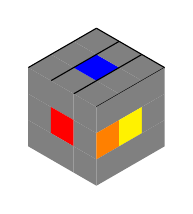
\begin{tikzpicture}[scale=1.0]
\drawtop{gray}{gray}{gray}{gray}{blue}{gray}{gray}{gray}{gray}
\drawleft{gray}{gray}{gray}{gray}{red}{gray}{gray}{gray}{gray}
\drawright{gray}{gray}{gray}{orange}{yellow}{gray}{gray}{gray}{gray}
\end{tikzpicture}
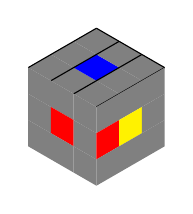
\begin{tikzpicture}[scale=1.0]
\drawtop{gray}{gray}{gray}{gray}{blue}{gray}{gray}{gray}{gray}
\drawleft{gray}{gray}{gray}{gray}{red}{gray}{gray}{gray}{gray}
\drawright{gray}{gray}{gray}{red}{yellow}{gray}{gray}{gray}{gray}
\end{tikzpicture}
\end{center}

Add 64 to \emph{solution number}.

\step

%Orientation of the 8th edge

\begin{center}
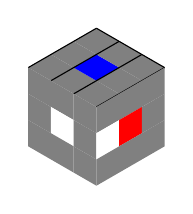
\begin{tikzpicture}[scale=1.0]
\drawtop{gray}{gray}{gray}{gray}{blue}{gray}{gray}{gray}{gray}
\drawleft{gray}{gray}{gray}{gray}{white}{gray}{gray}{gray}{gray}
\drawright{gray}{gray}{gray}{white}{red}{gray}{gray}{gray}{gray}
\end{tikzpicture}
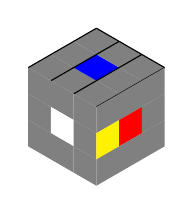
\begin{tikzpicture}[scale=1.0]
\drawtop{gray}{gray}{gray}{gray}{blue}{gray}{gray}{gray}{gray}
\drawleft{gray}{gray}{gray}{gray}{white}{gray}{gray}{gray}{gray}
\drawright{gray}{gray}{gray}{yellow}{red}{gray}{gray}{gray}{gray}
\end{tikzpicture}
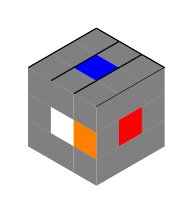
\begin{tikzpicture}[scale=1.0]
\drawtop{gray}{gray}{gray}{gray}{blue}{gray}{gray}{gray}{gray}
\drawleft{gray}{gray}{gray}{gray}{white}{orange}{gray}{gray}{gray}
\drawright{gray}{gray}{gray}{gray}{red}{gray}{gray}{gray}{gray}
\end{tikzpicture}
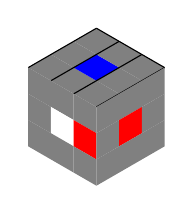
\begin{tikzpicture}[scale=1.0]
\drawtop{gray}{gray}{gray}{gray}{blue}{gray}{gray}{gray}{gray}
\drawleft{gray}{gray}{gray}{gray}{white}{red}{gray}{gray}{gray}
\drawright{gray}{gray}{gray}{gray}{red}{gray}{gray}{gray}{gray}
\end{tikzpicture}
\end{center}

Add 128 to \emph{solution number}.

\step

%Orientation of the 9th edge

\begin{center}
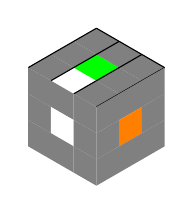
\begin{tikzpicture}[scale=1.0]
\drawtop{gray}{gray}{gray}{white}{green}{gray}{gray}{gray}{gray}
\drawleft{gray}{gray}{gray}{gray}{white}{gray}{gray}{gray}{gray}
\drawright{gray}{gray}{gray}{gray}{orange}{gray}{gray}{gray}{gray}
\end{tikzpicture}
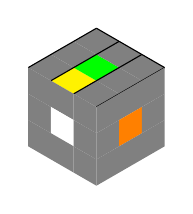
\begin{tikzpicture}[scale=1.0]
\drawtop{gray}{gray}{gray}{yellow}{green}{gray}{gray}{gray}{gray}
\drawleft{gray}{gray}{gray}{gray}{white}{gray}{gray}{gray}{gray}
\drawright{gray}{gray}{gray}{gray}{orange}{gray}{gray}{gray}{gray}
\end{tikzpicture}
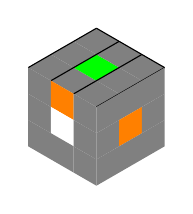
\begin{tikzpicture}[scale=1.0]
\drawtop{gray}{gray}{gray}{gray}{green}{gray}{gray}{gray}{gray}
\drawleft{gray}{orange}{gray}{gray}{white}{gray}{gray}{gray}{gray}
\drawright{gray}{gray}{gray}{gray}{orange}{gray}{gray}{gray}{gray}
\end{tikzpicture}
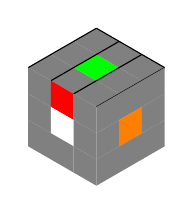
\begin{tikzpicture}[scale=1.0]
\drawtop{gray}{gray}{gray}{gray}{green}{gray}{gray}{gray}{gray}
\drawleft{gray}{red}{gray}{gray}{white}{gray}{gray}{gray}{gray}
\drawright{gray}{gray}{gray}{gray}{orange}{gray}{gray}{gray}{gray}
\end{tikzpicture}
\end{center}

Add 256 to \emph{solution number}.

\step

%Orientation of the 10th edge

\begin{center}
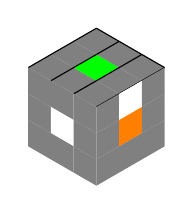
\begin{tikzpicture}[scale=1.0]
\drawtop{gray}{gray}{gray}{gray}{green}{gray}{gray}{gray}{gray}
\drawleft{gray}{gray}{gray}{gray}{white}{gray}{gray}{gray}{gray}
\drawright{gray}{white}{gray}{gray}{orange}{gray}{gray}{gray}{gray}
\end{tikzpicture}
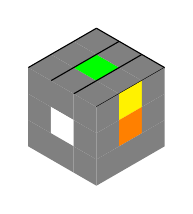
\begin{tikzpicture}[scale=1.0]
\drawtop{gray}{gray}{gray}{gray}{green}{gray}{gray}{gray}{gray}
\drawleft{gray}{gray}{gray}{gray}{white}{gray}{gray}{gray}{gray}
\drawright{gray}{yellow}{gray}{gray}{orange}{gray}{gray}{gray}{gray}
\end{tikzpicture}
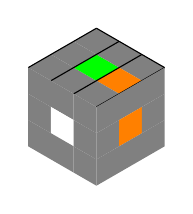
\begin{tikzpicture}[scale=1.0]
\drawtop{gray}{gray}{gray}{gray}{green}{gray}{gray}{orange}{gray}
\drawleft{gray}{gray}{gray}{gray}{white}{gray}{gray}{gray}{gray}
\drawright{gray}{gray}{gray}{gray}{orange}{gray}{gray}{gray}{gray}
\end{tikzpicture}
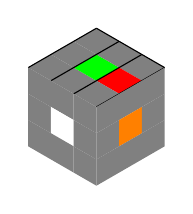
\begin{tikzpicture}[scale=1.0]
\drawtop{gray}{gray}{gray}{gray}{green}{gray}{gray}{red}{gray}
\drawleft{gray}{gray}{gray}{gray}{white}{gray}{gray}{gray}{gray}
\drawright{gray}{gray}{gray}{gray}{orange}{gray}{gray}{gray}{gray}
\end{tikzpicture}
\end{center}

Add 512 to \emph{solution number}.

\step

%Orientation of the 11th edge
%The final edge
%No need to check the 12th edge
%Edge parity is always even

\begin{center}
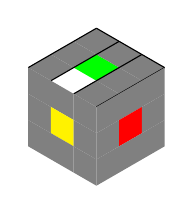
\begin{tikzpicture}[scale=1.0]
\drawtop{gray}{gray}{gray}{white}{green}{gray}{gray}{gray}{gray}
\drawleft{gray}{gray}{gray}{gray}{yellow}{gray}{gray}{gray}{gray}
\drawright{gray}{gray}{gray}{gray}{red}{gray}{gray}{gray}{gray}
\end{tikzpicture}
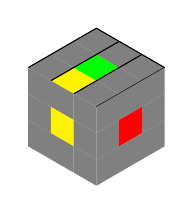
\begin{tikzpicture}[scale=1.0]
\drawtop{gray}{gray}{gray}{yellow}{green}{gray}{gray}{gray}{gray}
\drawleft{gray}{gray}{gray}{gray}{yellow}{gray}{gray}{gray}{gray}
\drawright{gray}{gray}{gray}{gray}{red}{gray}{gray}{gray}{gray}
\end{tikzpicture}
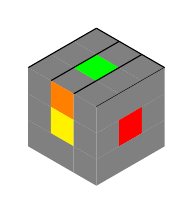
\begin{tikzpicture}[scale=1.0]
\drawtop{gray}{gray}{gray}{gray}{green}{gray}{gray}{gray}{gray}
\drawleft{gray}{orange}{gray}{gray}{yellow}{gray}{gray}{gray}{gray}
\drawright{gray}{gray}{gray}{gray}{red}{gray}{gray}{gray}{gray}
\end{tikzpicture}
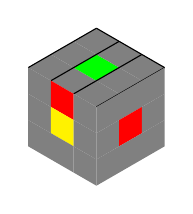
\begin{tikzpicture}[scale=1.0]
\drawtop{gray}{gray}{gray}{gray}{green}{gray}{gray}{gray}{gray}
\drawleft{gray}{red}{gray}{gray}{yellow}{gray}{gray}{gray}{gray}
\drawright{gray}{gray}{gray}{gray}{red}{gray}{gray}{gray}{gray}
\end{tikzpicture}
\end{center}

Add 1024 to \emph{solution number}.

\end{document}

